
\section{.Forty-Fives grundlegendste Regeln}\label{sec:grundlegenste-regeln}

\renewcommand{\kapitelautor}{Autor: Irgendwer} % todo: replace

%
.Forty-Five ist ein digitales Kartenspiel des Subgenres des Rogue-like Deckbuilders. %TODO: Quelle für Erklärung
Der Spieler bewegt sich über eine Map, die prozentual generiert ist, sammelt Karten und benutzt diese Karten,
um Gegner zu bekämpfen. Sollte der Spieler einen Kampf verlieren, stirbt er, seine gesammelten Karten
gehen verloren und er startet wieder am Anfang. Da es sich jedoch um ein "Rogue-Lite" handelt und nicht um ein "Rogue-Like",
gibt es eine Art von speicherbarem Fortschritt, den der Spieler in sein nächstes Leben mitnehmen kann.
Ein Durchlauf bzw. ein Leben des Spielers wird als "Run" bezeichnet. Ein Run endet mit dem Tod des Spielers.
Während der Entwicklung wurden jene Elemente, die in das nächste Leben übergehen, als "Rogue-Lite-Elemente" bezeichnet.



%zuerst erklären was roads und so sind????
\subsection{.Forty-Fives Rogue-Lite-Elemente}\label{rogue_lite_elemente}

Um das Spielerlebnis des Spielers nicht allzu frustrierend zu gestalten, wurden zwei verschiedene Mechaniken eingeführt.
Bei der ersten Mechanik handelt es sich um die Erhöhung der maximalen Lebenspunkte des Spielers bei Heilpunkten im Spiel. Der Spieler hat die Möglichkeit
sich zu entscheiden, ob er sich lieber nur für diesen Run heilt und dafür auch eine größere Menge an Lebenspunkten erhält, oder ob er
lieber in das Erhöhen seiner Lebenspunktkapazität investiert. Bei letzterem handelt es sich natürlich um eine kleinere Zahl als bei der anderen Wahl.
Dies dient dazu, dem Spieler die Entscheidung offen zu halten, entweder etwas Langwieriges aber Bleibendes zu investieren oder lieber noch einmal ordentlich
Lebenspunkte aufzutanken, was bei der zweiten Mechanik ins Spiel kommt. %todo quelle füg max hp und hp generell

\begin{figure}[H]
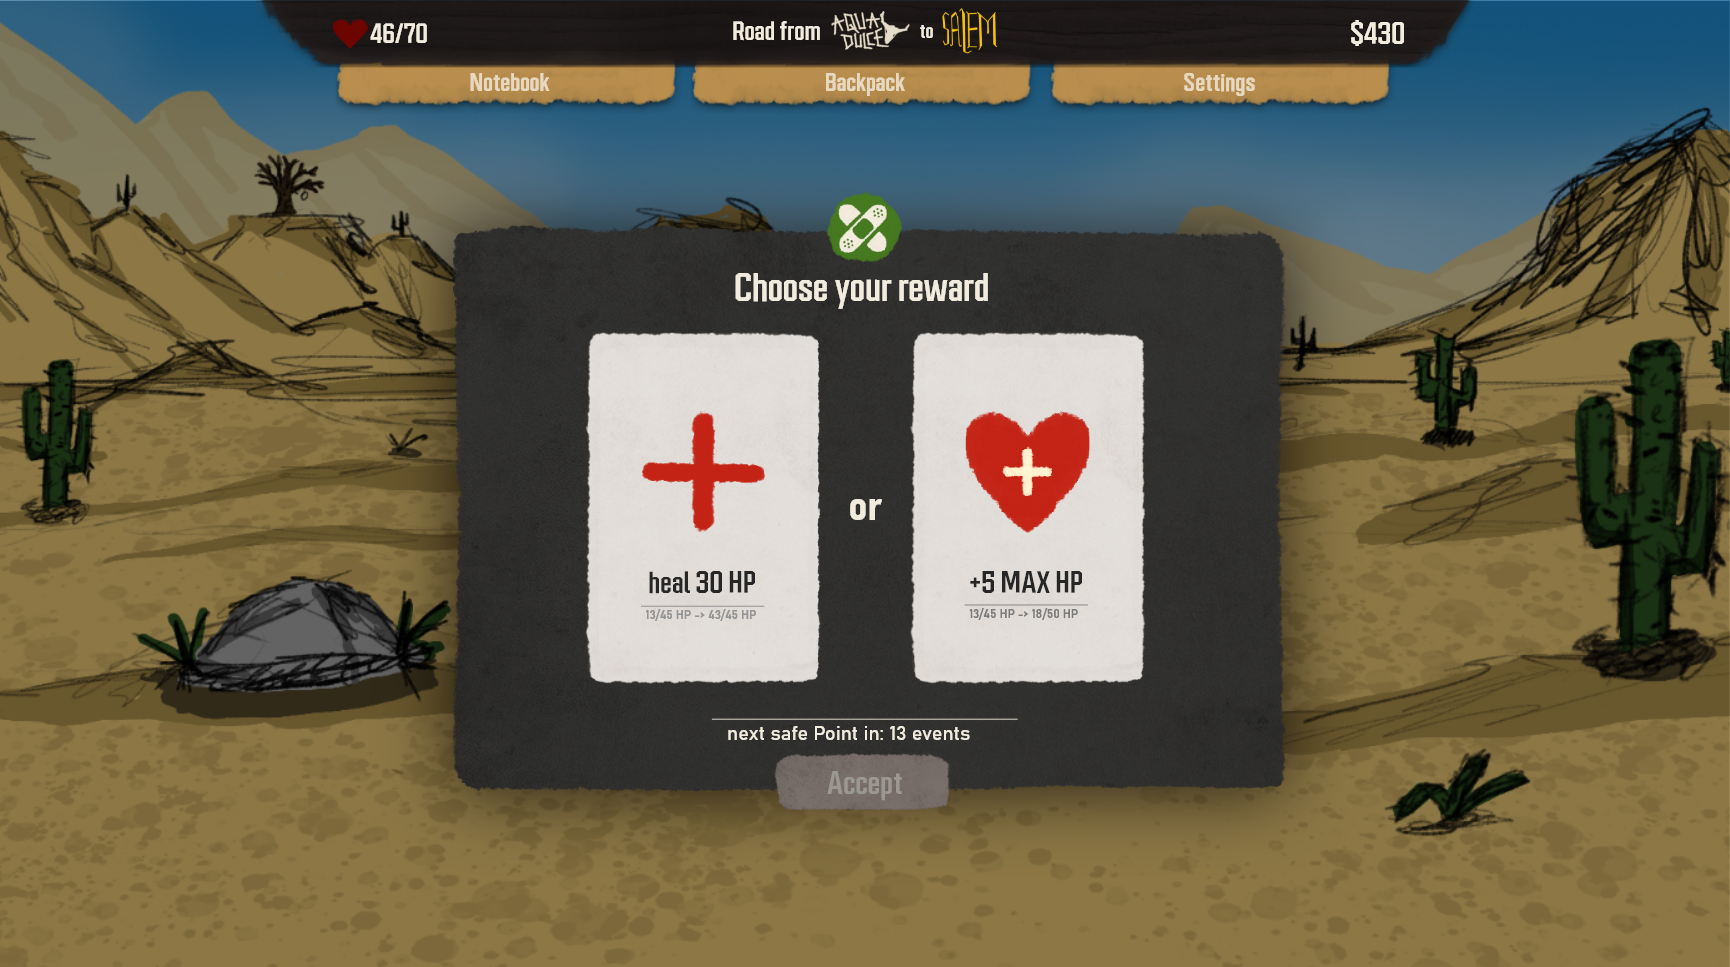
\includegraphics[width=\textwidth]{healeventgrafic.png}
\caption{Ein Heilevent}
\end{figure}


Schafft der Spieler einen Abschnitt des Spiels, also eine sogenannte Road, werden seine bis zu dem Zeitpunkt gesammelten Karten
gespeichert und sind ab dann selbst nach einem Tod jederzeit zugänglich und spielbar.

\begin{figure}[H]
    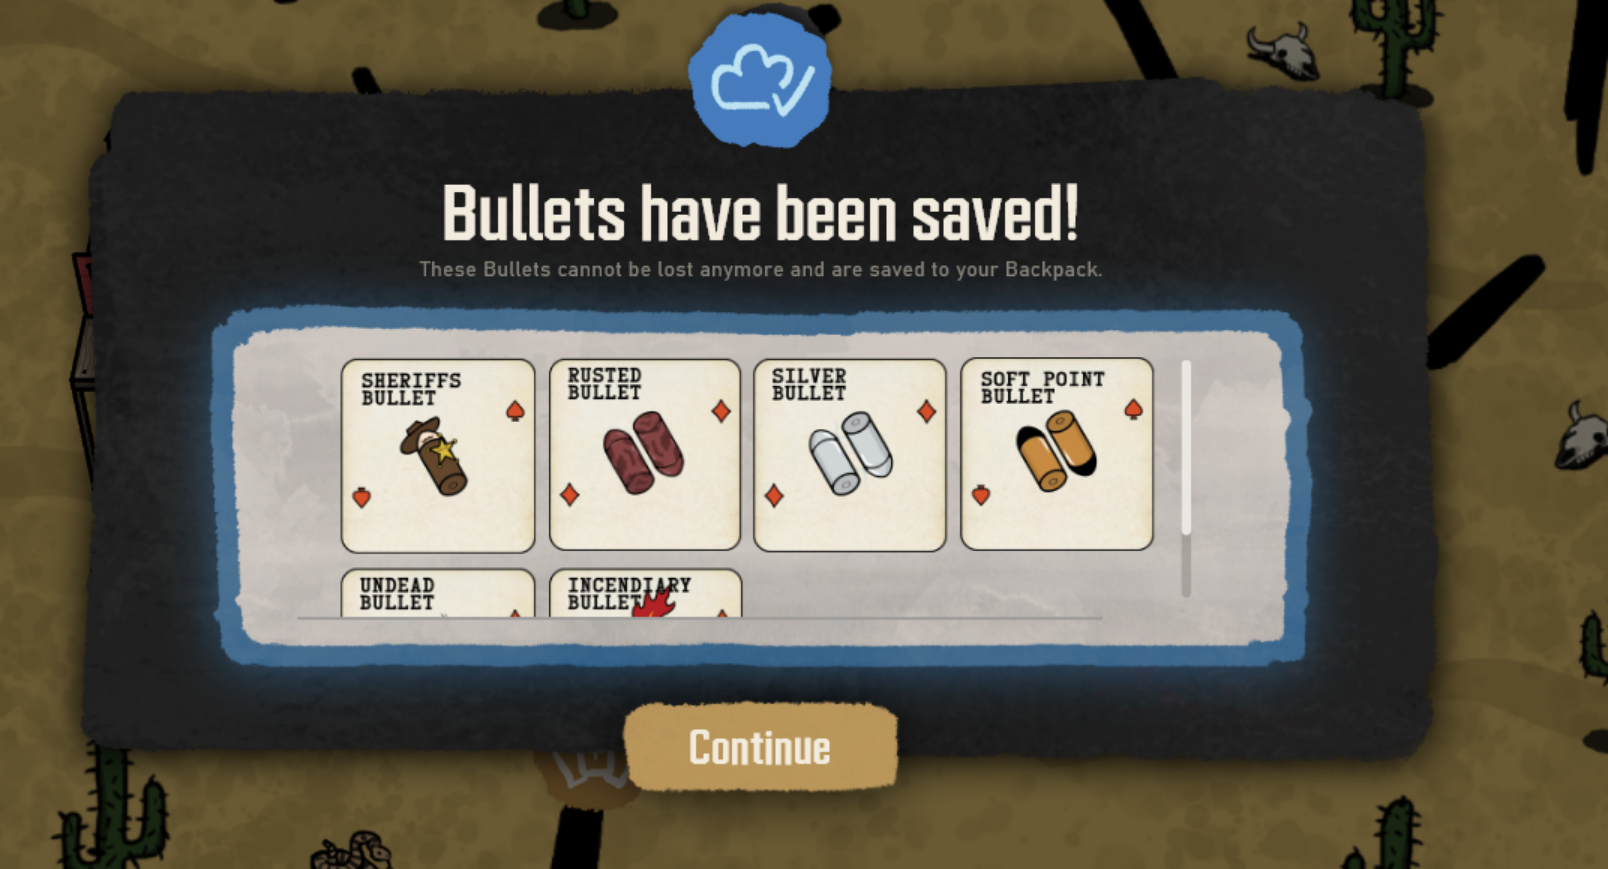
\includegraphics[width=\textwidth]{bulletssavedPopup.png}
    \caption{Das Popup, welches am Ende der Road erscheint um zu zeigen welche Karten gespeichert wurden}
\end{figure}


\begin{figure}[H]
    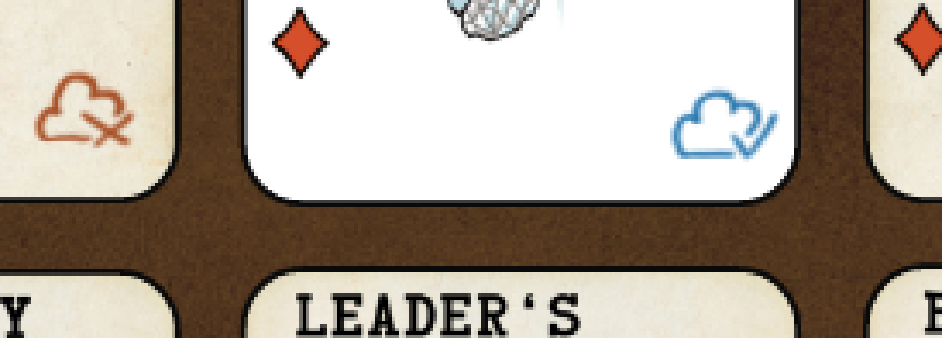
\includegraphics[width=\textwidth]{bulletsaved.png}
    \caption{Karten die gespeichert wurden, werden mit diesem Symbol in der rechten unteren Ecke der Karte markiert.}
\end{figure}

Verknüpft mit der ersten Mechanik
hat der Spieler die Möglichkeit, sich dazu zu entscheiden, seine Leben wieder aufzuheilen und das Ende der Road anzustreben.
Ist er der Meinung, es sowieso nicht mehr zu dem Abschnittsende zu schaffen, wählt er die Erhöhung der maximalen
Lebenspunkte, um so zumindest einen Vorteil in den nächsten Runs zu haben. Der Spieler muss also das Risiko und die
Belohnung abwägen und daran entscheiden, welche Wahl er trifft.



\subsection{Das Sammeln der Karten}\label{sammeln_der_Karten}

Nach jedem überlebten Kampf bekommt der Spieler eine neue Karte. Er bekommt drei verschiedene Karten zur Auswahl gezeigt und darf sich eine davon aussuchen.
Außerdem gibt es auf der Map verteilt noch zusätzliche Events, die der Spieler aufsuchen kann, um seine Sammlung zu erweitern.

\begin{figure}[H]
    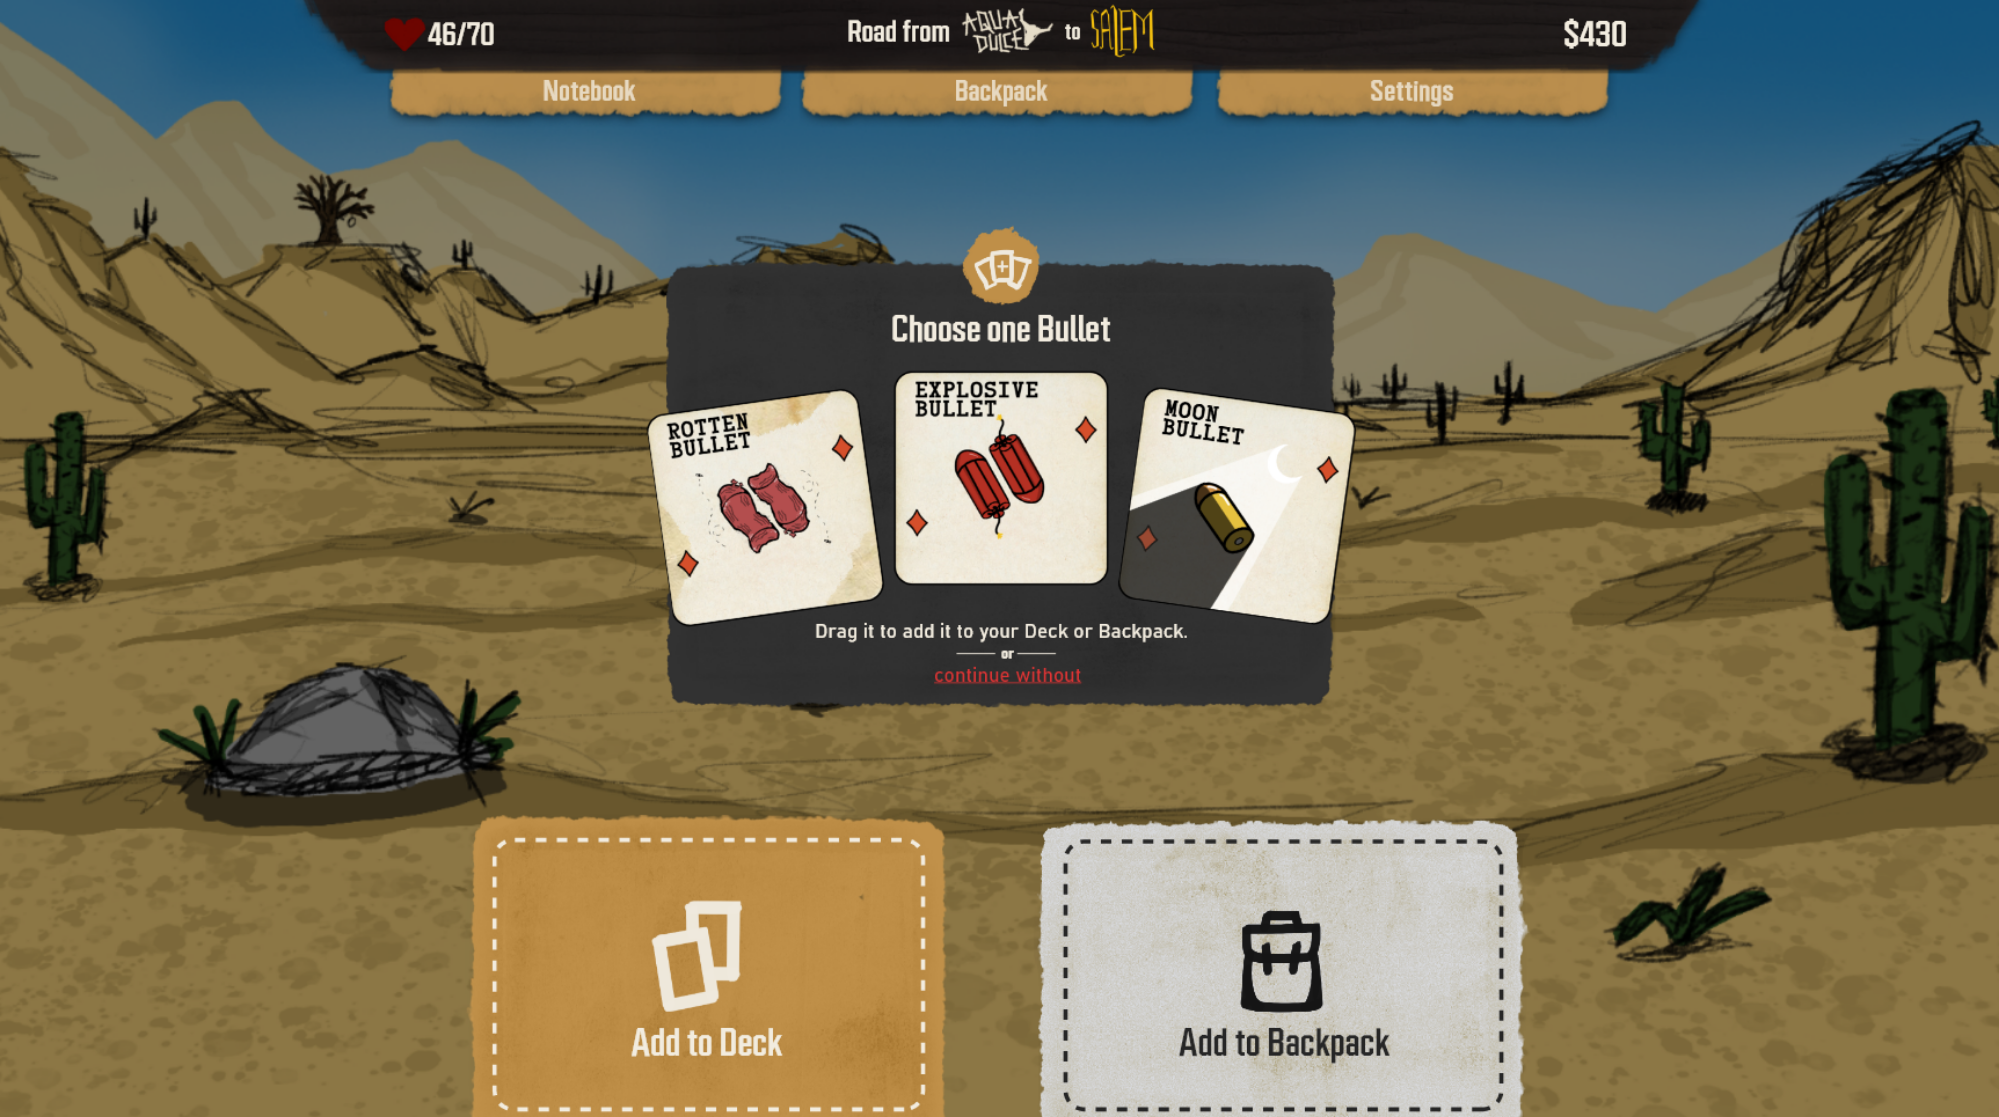
\includegraphics[width=\textwidth]{choosebullet.png}
    \caption{Eine von drei Karten kann ausgesucht werden.}
\end{figure}

Das bringt nicht nur wieder eine Entscheidung des Spielers mit sich, die den Verlauf des Runs ändert, sondern bringt auch mehr Abwechslung,
da der Spieler nicht immer nur die Karten nehmen kann, die er gerne hätte. Es bringt auch eine Art Entdeckerlust mit sich, da der Spieler
auf diese Weise natürlich die Karten erst nach und nach sieht und nicht alle gleich auf einmal (siehe z.B. Magic Arena, wo alle Karten sofort in einer eigenen Liste zugänglich sind). %todo: Quelle

"It is not that players build a deck in order to play the game, it is that they play the game in order to build a deck."\cite{zitatdeckbuilding}

und zwingt den Spieler mit begrenzter Wahl und Ressourcen das Beste daraus zu machen. Diese Designpolitik wird beim Design der Karten beachtet und wird zu einem späteren Zeitpunkt genauer erläutert %TODO macht man das so?
Viele Rogue-like Deckbuilder haben ein ähnliches System. Inspiriert wurde das Sammeln der Karten in ".Forty-Five" von Spielen wie Inscription und Slay the Spire,
hat jedoch einen großen Unterschied. Anders als in z.B. Slay the Spire können Karten ganz einfach aus dem Kartendeck entfernt werden, nachdem sie einmal ausgewählt wurden.
Karten können aus dem Deck in den Backpack verschoben werden und ermöglichen dadurch ein flexibleres Spielerlebnis.\cite{slaythespire, inscryption}


\begin{figure}[H]
    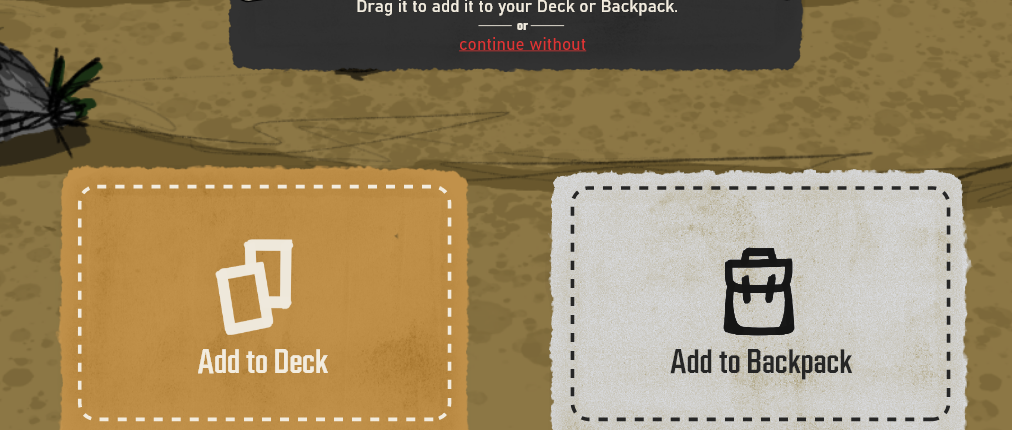
\includegraphics[width=\textwidth]{deckandbackpack.png}
    \caption{Eine Karte kann entweder gleich in das Deck gegeben werden, und ist damit im Kampf aktiv, oder in den Backpack also die reserve verschoben werden.}
\end{figure}

\subsection{Der Backpack und das Deck}\label{backpack_and_deck}
\begin{infoBox}
Note: Zu diesem Zeitpunkt geht es nicht um die Designprinzipien hinter dem Deck und den Karten,
sondern nur um die Erklärung der grundlegenden Mechaniken. Das Gamedesign wird zu einem späteren Zeitpunkt beschrieben.
\end{infoBox}
Der Backpack und das Deck dienen beide als Speicherort für Karten, mit dem Unterschied, dass die Karten im Deck aktiv im
Kampf eingesetzt werden und die Karten im Backpack mehr als Reserve gelten.
Karten können frei zwischen den beiden verschoben werden, solange die festgelegte Mindestanzahl an Karten im Deck eingehalten wird.
Da Forty-Five viele verschiedene Strategien bietet, gibt es mehrere Decks, zwischen denen man einfach wechseln kann.
Das hat zur Folge, dass der Spieler nicht immer ein Deck zerlegen muss, um eine andere Strategie auszutesten.

\begin{figure}[H]
    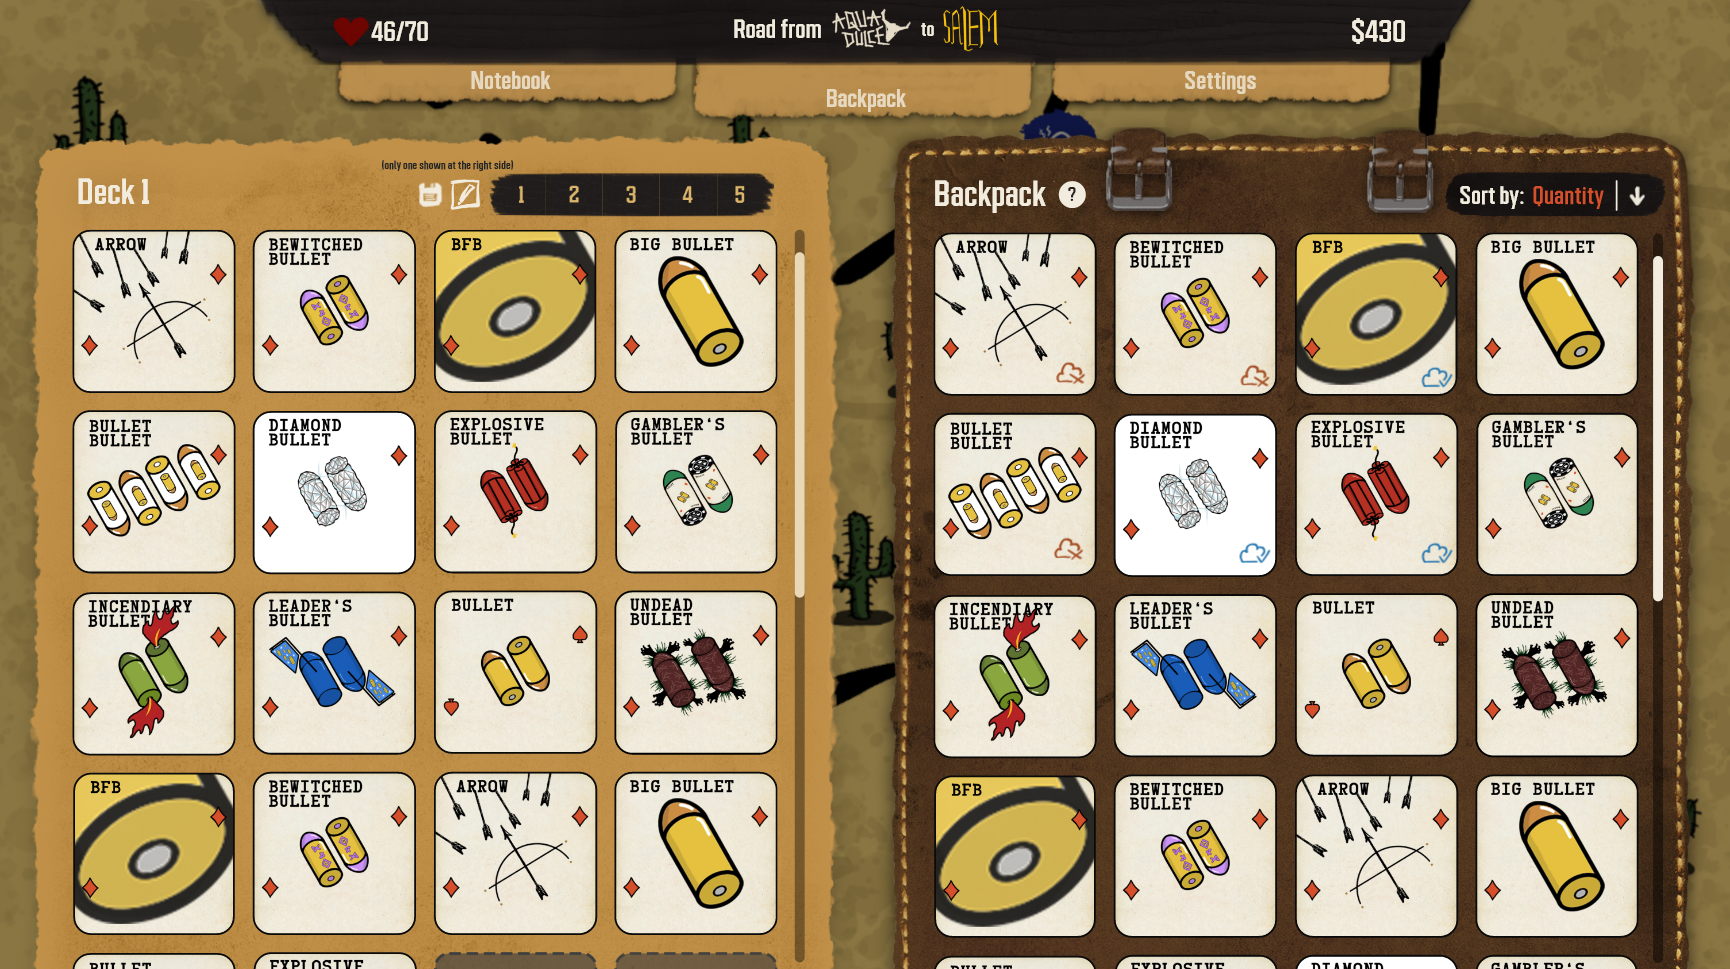
\includegraphics[width=\textwidth]{deckview.png}
    \caption{Ansicht des Decks und des Backpacks}
\end{figure}

\begin{figure}[H]
    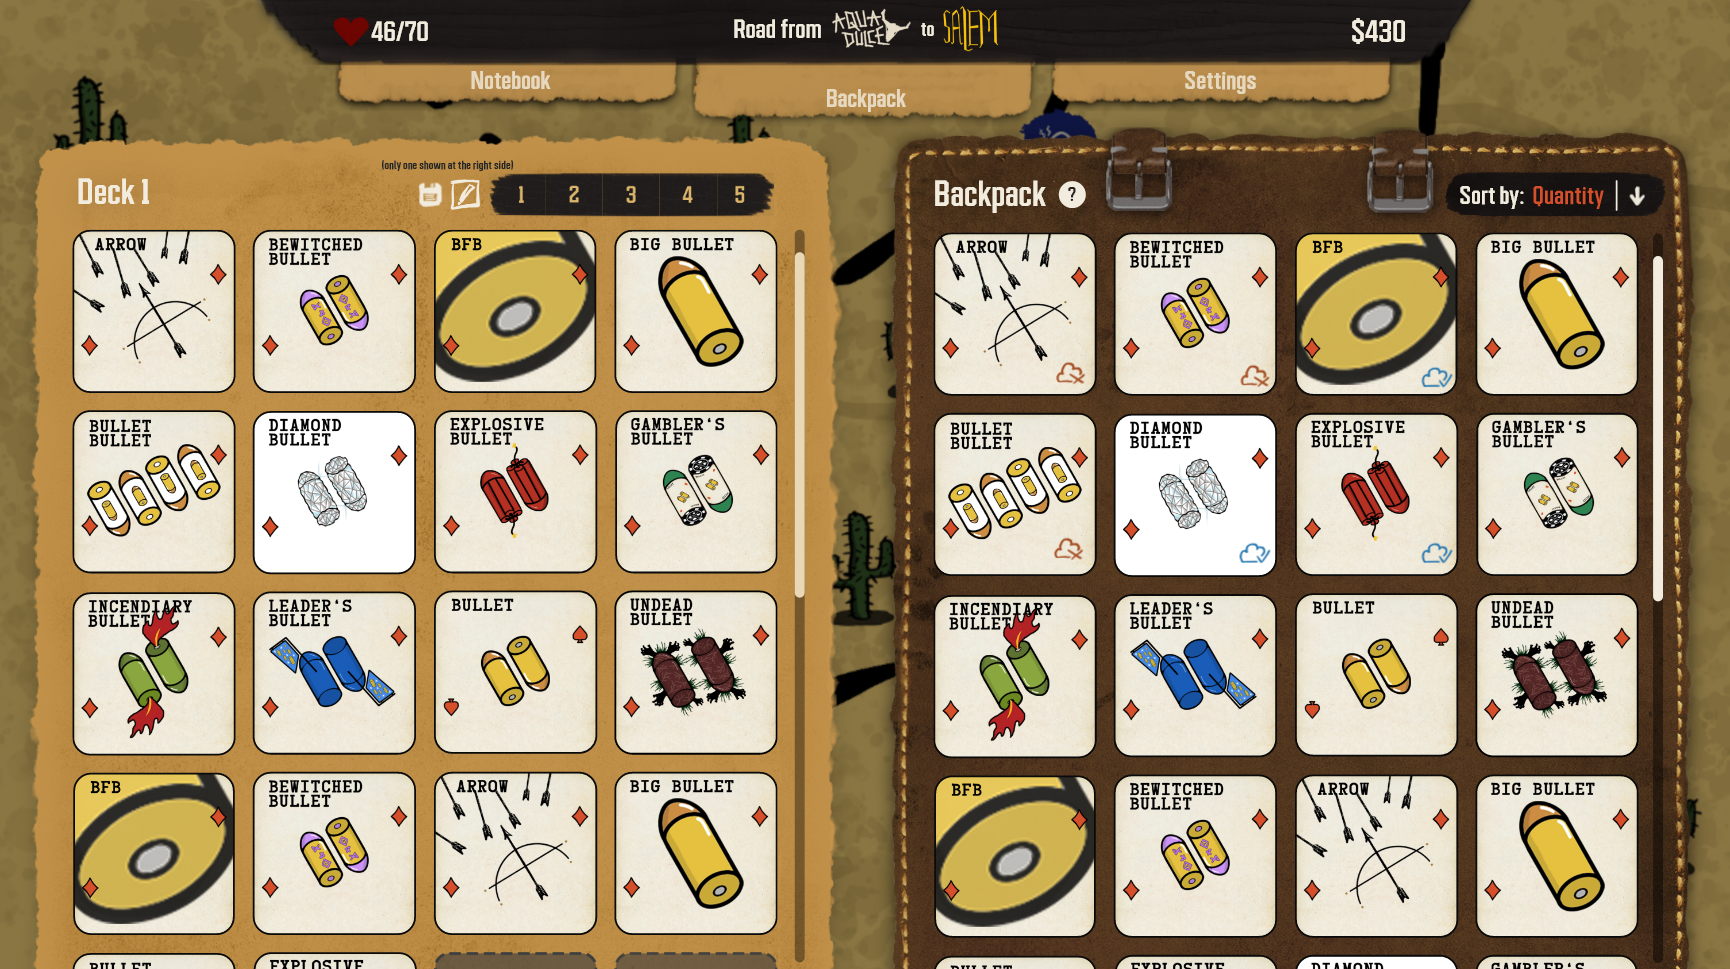
\includegraphics[width=\textwidth]{deckview.png}
    \caption{Ui für das Wechseln des Deckes}
\end{figure}


Außerdem können Decks umbenannt werden, um besser wiedergefunden und erkannt zu werden.

Karten können im Backpack nach Kriterien wie Kosten oder Namen auf- und absteigend sortiert werden.

\begin{figure}[H]
    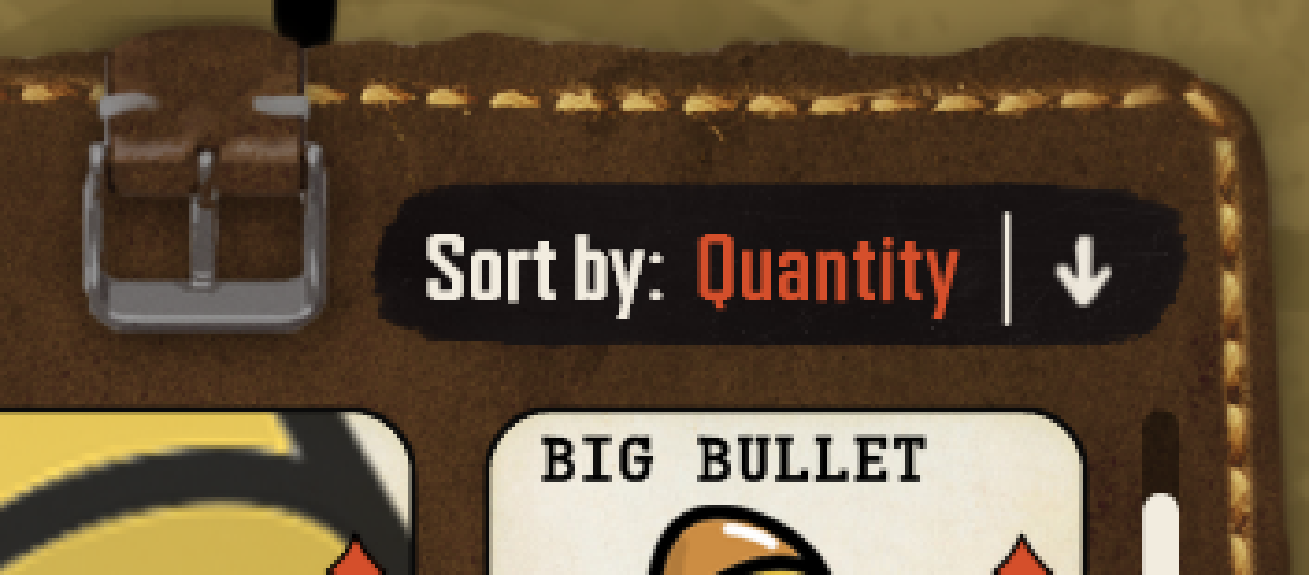
\includegraphics[width=\textwidth]{sortdeck.png}
    \caption{Durch klicken kann durch verschiedene Sortierungs-Möglichkeiten durchgewechselt werden.}
\end{figure}

Sammelt der Spieler eine neue Karte, kann er sich entscheiden, ob er die Karte gleich seinem Deck oder doch eher seinem
Backpack hinzufügen möchte.
Der Backpack und das Deck ermöglichen es dem Spieler, Karten, die er gesammelt hat, aus dem Deck zu nehmen und damit
nicht zu verwenden, sowie Decks zu bauen, die zu einer Strategie passen.
Startet der Spieler nun einen Kampf, wird das zuletzt ausgewählte Deck verwendet.


\subsection{Der Kampf}\label{backpack_and_deck}
%grundsätzliche sachen wie reserves, gegner und spieler, gewonnen wenn gegner tod usw karten am anfang ziehe zwei karten am anfang vom turn

Während der Spieler über die Map reist, sind Kämpfe unausweichlich.

\begin{figure}[H]
    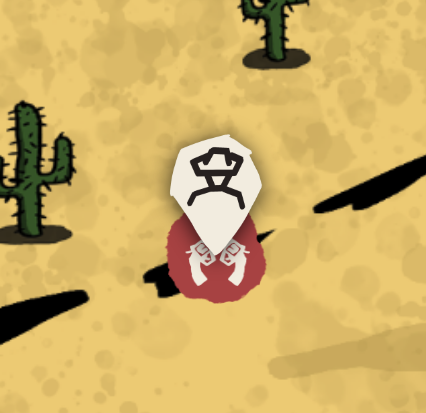
\includegraphics[width=\textwidth]{playericon.png}
    \caption{Kämpfe werden auf der Map durch zwei gekreuzte Revolver dargestellt. Um weiter auf der Map fortzuschreiten müssen sie absolviert werden.}
\end{figure}

Gekämpft wird mit den gesammelten Karten, mit dem Ziel, den oder die Gegner zu besiegen und dabei so wenig Lebenspunkte
wie möglich zu verlieren bzw. nicht zu sterben. Gewonnen hat der Spieler, wenn alle Gegner besiegt wurden.
Ein Kampf ist aufgeteilt in Züge. Immer abwechselnd ist entweder der Spieler oder der Gegner dran. Am Anfang des Kampfes
werden eine vordefinierte Anzahl an Karten vom Deck des Spielers gezogen. %todo die genaue Anzahl fehlt noch (5 oder 6?)
Anschließend hat der Spieler die Möglichkeit, nach Belieben seinen Zug auszuführen. Ein Spielerzug wird mit dem "Holster"
Button beendet, und das Betätigen des Knopfes startet den automatischen Ablauf des Gegnerzuges. Der Gegner führt eine mehr oder weniger zufällige Aktion aus, und danach ist wieder der Zug des Spielers.
Am Start des Zuges des Spielers werden zwei Karten vom Deck gezogen. Pro Zug des Spielers stehen dem Spieler 4 "Reserves"
zur Verfügung. Diese werden jeweils auch am Anfang des Zuges wieder auf die maximale Anzahl aufgefüllt.
Reserves können dazu verwendet werden, Karten zu bezahlen und damit auch zu spielen.

\begin{figure}[H]
    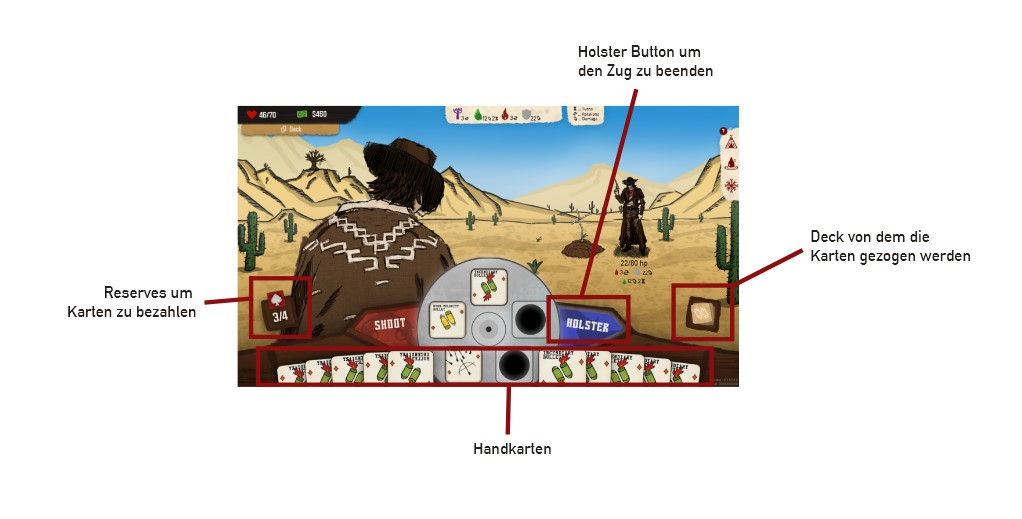
\includegraphics[width=\textwidth]{turngrafic.jpg}
    \caption{Durch die Kampf Ui werden alle wichtigen Informationen an den Spieler weitergegeben.}
\end{figure}



\subsection{Karten}\label{Karten}
Karten in \FF sind Bullets. Jede Bullet hat einen Kosten, die bezahlt werden müssen, um die Karte zu spielen.
Die Reserven, die für die Bullet benötigt werden, werden automatisch bezahlt, WENN der Spieler sich die Bullet leisten kann, sobald die Bullet gespielt wird.
Das Management von diesen Reserves und die Reihenfolge, in der man die Karten spielt, ist wichtig, um besser in Forty-Five zu werden. %TODO Mehr dazu ist im Gamedesign.
Jede Bullet hat außerdem einen Damage-Wert, welcher angibt, wie viele Lebenspunkte dem Gegner durch die Karte abgezogen werden,
falls die Karte auf den Gegner geschossen wird.

\begin{figure}[H]
    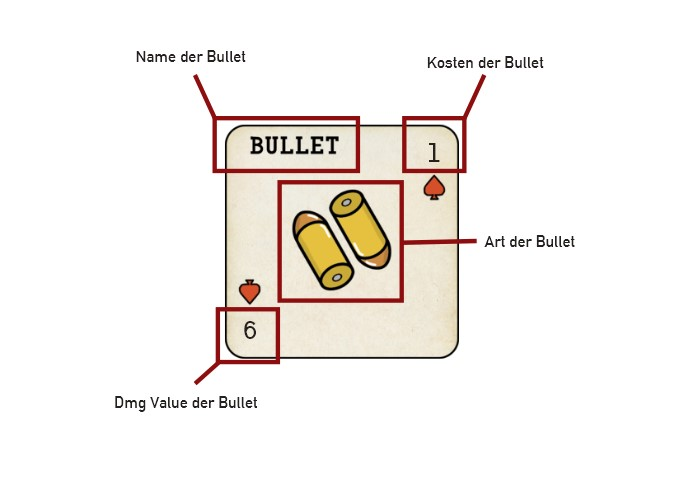
\includegraphics[width=\textwidth]{bulletgrafic.jpg}
    \caption{Die wichtigsten Infos werden auf der Karte angezeigt.}
\end{figure}

Fast alle Karten haben außerdem einen einzigartigen Effekt,
welcher angesehen werden kann, indem der Spieler mit der Maus über die gewünschte Bullet hovert.
In dem Popup, welches nach dem Hovern sichtbar ist, befinden sich die Infos zu dem Effekt der Karte,
dazu gehört fast immer ein Trigger und der Effekt selbst.

\begin{figure}[H]
    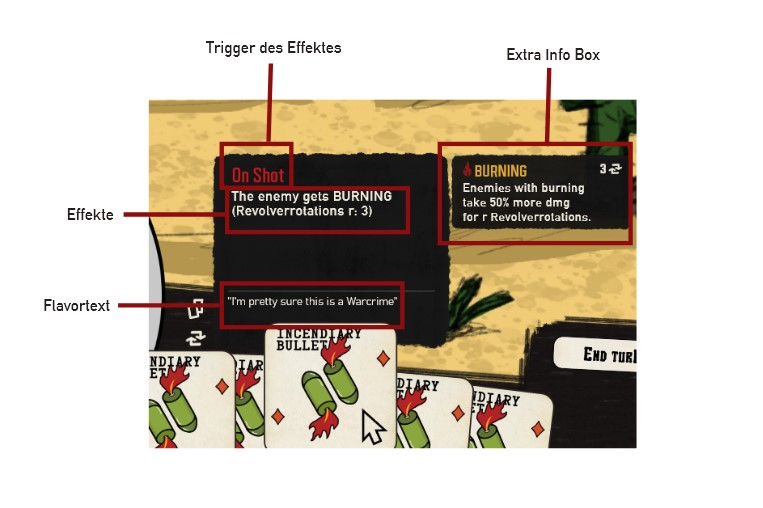
\includegraphics[width=\textwidth]{hovergrafic.jpg}
    \caption{Um genauere Infos über den Effekt und Hintergründe der Karte zu erhlaten, kann man über sie drüber hovern.}
\end{figure}


Der Trigger gibt an, wann sich der Effekt aktiviert. Es gibt verschiedene Trigger, wie zum Beispiel das Aktivieren des Effektes beim Spielen der Bullet. %TODO siehe mehr später bei trigger
Zusätzlich zu dem Effekt und dem Trigger steht bei vielen Karten außerdem noch ein Flavortext dabei.
Ein Flavortext ist ein Spruch, der der Bullet ein wenig Kontext hinzufügt.
Dies kann passieren durch einen dummen Spruch, einen Witz, eine Anspielung oder einen story- bzw. worldbuilding-relevanten Text.
Falls nötig werden relevante Infos zu dem Effekt in einer extra Box rechts oder links angezeigt.
Bullets werden, wenn sie gespielt werden in den Revolver geladen.

\subsection{Der Revolver}\label{der_revolver}
Der Revolver ist das Spielfeld von \FF, in welches die Bullets platziert bzw. "geladen" werden.
Mithilfe von Drag and Drop kann der Spieler die Karte aus seiner Hand in den Revolver legen.
Dies ist das bereits erwähnte Spielen einer Karte, zu dem auch das Bezahlen gehört.
Der genaue Ablauf des Spielens einer Karte ist wie folgt:
Drag and Drop in den gewünschten Revolverplatz > Bezahlen der Reserven, Abbruch falls nicht genug Reserven vorhanden sind > Platzieren der Bullet > möglicherweise Aktivieren von Triggern, falls die Bullet einen Effekt hat, der einen On-Placedown Trigger hat.


Der Revolver besteht aus 5 Kammern bzw. Feldern, in die Bullets geladen werden können.
Sie sind von 1-5 nummeriert. %TODO Bild und noch Umdrehen von 5 zu 1
Der Revolver kann von dem Spieler geschossen werden. Wenn geschossen wird, wird die Bullet in der obersten Kammer auf den Gegner geschossen.
Verlässt sie den Revolver, verliert der Gegner Lebenspunkte in Höhe des Dmg Value der geschossenen Bullet.
Die Bullet wird unter das Deck gelegt und der Revolver dreht sich einmal nach rechts.

\begin{figure}[H]
    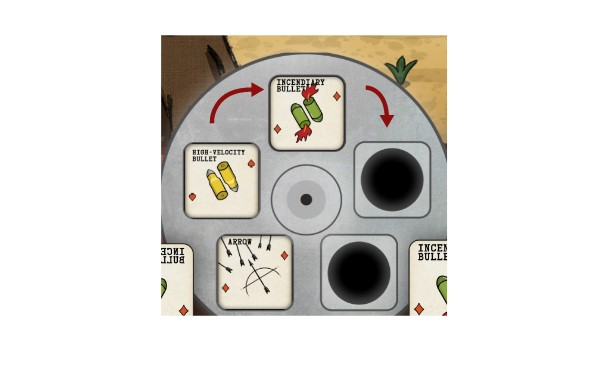
\includegraphics[width=\textwidth]{rotategrafic.jpg}
    \caption{Der Revolver dreht sich normalerweiße nach dem feuern des Revolvers einmal nach rechts.}
\end{figure}


Die Revolverrotation ist ein wichtiger Teil von Forty-Five, da man das Placement der Bullets im Revolver sich genau überlegen muss,
um das Meiste aus seinen Bullets herauszuholen. %todo mehr in Game Design.
Es gibt außerdem einen Trigger, welcher aktiviert wird, wenn die Karte geschossen wird,
namens On-Shot. Zusätzlich gibt es Karten mit Effekten, welche die Revolverrotation verändern, wie z.B. Bewitched Bullet,
welche den Revolver nach links statt nach rechts rotiert.

Die Komplexität von \FF kommt vom Meistern des Revolvers.
Das strategische Platzieren von Bullets, die Reihenfolge der Bullets und das Verstehen, wie eine Revolverrotation sich auf Bullets,
den Spieler oder den Gegner auswirkt. Die gerade erwähnte Bewitched Bullet kann zum Beispiel dazu verwendet werden, Karten,
welche davon profitieren, lange im Revolver zu bleiben, weiter von dem Schießen wegzuschieben. Bullet zum Beispiel fügt dem Gegner Schaden zu,
wenn sich Bullet rotiert im Revolver. %TODO BILDER!!!
Bewitched Bullet kann dazu verwendet werden, zwei zusätzliche Rotationen rauszuholen, indem man den Revolver einmal nach
links dreht, bevor Bullet den Revolver verlässt. Bewitched Bullet kann zum Beispiel auch zum Einschieben von Bullets verwendet
werden und so weiter und so fort. Die Kombinationsmöglichkeiten sind endlos, und fast jeder Effekt einer Bullet kann mit dem einer
anderen Bullet verknüpft werden.



%slots rotationen usw karten weg wenn shot und karten unters deck gelegt wenn shot usw


\subsection{Zonen}\label{backpack_and_deck}
%probbaly unnötig

\subsection{Der Gegner}\label{der_gegner}
Der Gegner, auf den die Bullets des Spielers geschossen werden, besteht aus mehreren Komponenten.
Genau wie der Spieler verfügt der Gegner über einen HP-Wert. Wenn der Wert null erreicht, stirbt der Gegner.
Nachdem der Spieler "End turn" gedrückt hat, beendet er seinen Zug und der Gegner ist dran. Während dem Zug des Spielers
zeigt der Gegner die Aktion an, die er in seinem Zug ausführen wird.
Gegneraktionen werden "zufällig ausgewählt aus dem Pool von Aktionen des Gegners.
Jedoch wurden die Aktionen angepasst, um nicht nur Fairness zu garantieren,
sondern auch eine Balance zwischen zu leicht und zu schwer zu finden.
Mehr zum Balancen der Gegner kann in 07 Gamedesign nachgelesen werden.


Sobald der Gegner dran ist, wird die Aktion automatisch ausgeführt. Je nach Gegnertyp gibt es andere Aktionen,
die ein Gegner ausführen kann. Universell ist jedoch die Aktion des Schadens zufügens.
Es gibt viele verschiedene Arten von Gegneraktionen, die dafür entwickelt wurden, mehr Abwechslung beim Bekämpfen der Gegner zu bieten.
Außerdem sollte noch erwähnt werden, dass es auch passieren kann, dass der Spieler gegen mehr als einen Gegner kämpft.
Ist das der Fall, sucht der Spieler das Ziel der Revolverschüsse, indem er auf den gewünschten Gegner klickt.
Dargestellt durch ein Symbol über dem Kopf des Gegners, sind die Aktionen weniger eine Reaktion auf den Spieler,
sondern es wird eher erwartet, dass der Spieler die Aktion des Gegners in das Planen seines Zuges miteinbezieht.
Bei der eben genannten Schadenaktion kann der Spieler darauf reagieren und Schaden verhindern, indem er die Karte parried.

\subsection{Parrying}\label{parrying}
Das Parieren des Schadens, der vom Gegner verursacht wird, wird in \FF durch Bullet gemacht.
Die Idee dahinter ist, dass die eigene Bullet verwendet wird, um den Angriff des Gegners abzuhalten, indem man
seine Bullet gegen die des Gegners schießt.
Der Spieler bekommt die Wahl, ob er parrieren möchte oder nicht, was durch ein eigenes Popup während des gegnerischen Zugs geregelt wird.
Entscheidet sich der Spieler dazu zu parieren, wird dafür die Bullet im vordersten Slot verwendet.
Dann wird der Schadenswert des Gegners mit dem der Bullet substituiert. Ist der Schadenswert der Bullet größer als der des Gegners,
geht kein Schaden durch. Ist es andersrum, bekommt der Spieler so viel Schaden wie die Differenz ausmacht.
Es ist wichtig zu erwähnen, dass nicht geparriert werden muss, sollte der Spieler die Bullet lieber behalten wollen,
bzw. wenn er der Meinung ist, den Schaden einfach einzustecken zu können. Durch einen Parry geht die Bullet verloren,
es aktiviert keine Effekte und sie wird danach wieder unters Deck gelegt.


Als Zusatz gibt es Bullets, die einen defensiven Effekt haben, mit denen sich der Spieler zusätzlich schützen kann.

\subsection{Spezifische Regeln}\label{spezifische_regeln}

Es gibt ein paar zusätzliche Regeln in \FF, die nun angeführt werden.


Die erste ist der sogenannte Overkill-Schaden.
Die Regel besagt, dass jeglicher Schaden, der dem Gegner zugefügt wird, nachdem seine Lebenspunkte bereits unter 0 sind,
in Geld umgewandelt wird. Das Geld kann benutzt werden, um sich bei einem Shop weitere Karten zu kaufen.
Die Overkill-Regel gilt jedoch nur für den aktuellen Zug. Drückt der Spieler auf "End Turn", wird der Zug und der Kampf beendet.
Overkill-Cash ist nicht nur eine gute Möglichkeit, Belohnungen anhand der Leistung des Spielers zu berechnen,
sondern löst auch gleichzeitig folgendes Problem: In \FF ist der Aufbau des Revolvers und damit von Combos sehr wichtig.
Oft kommt es vor, dass der Spieler eine Combo aufgebaut hat, der Gegner jedoch einfach schneller tot ist.
Das ist nicht nur frustrierend, sondern gibt dem Spieler auch einfach keinen Grund, überhaupt starke Combos aufzubauen,
wenn er sich einmal über dem Standard-Gegnerschwierigkeitslevel befindet. Overkill-Schaden löst diese beiden Probleme.


Die zweite Regel bezieht sich auf das Schießen des Revolvers.
Die Regel besagt, dass, wenn der Revolver leer geschossen wird, also kein Bullet in der vordersten Kammer vorhanden ist,
der Spieler 5 Lebenspunkte Schaden erleidet. Das Wann, das Wo und das Wie ist das Wichtigste beim Bullet platzieren.
Einen Bullet in den hintersten oder ersten Slot zu platzieren, ist eine Entscheidung, die überlegt sein sollte.
Ohne diese Regel ist es jedoch möglich, Bullets, die man weiter hinten platziert hat, sofort wieder vorrotieren zu lassen,
was das gesamte Spielprinzip der Revolverdrehung ruinieren würde, da das Platzieren keine Konsequenzen hätte.
Es würde dazu führen, dass Bullets nacheinander einfach in den Revolver geladen werden, wo es gerade passt, und sofort
geschossen werden, da die Schussreihenfolge der Bullets ja sowieso egal ist. Jedoch wollten die Entwickler das Rotieren
des Revolvers ohne ein Bullet in dem vordersten Slot durch das Schießen nicht verbieten, sondern führten ein,
dass 5 Lebenspunkte abgezogen werden. Das bedeutet also, dass es im Notfall gemacht werden kann, z.B. falls es einmal für
eine Combo nötig ist, jedoch nicht durchgehend benutzt werden kann, da der Spieler durch das Abziehen der Lebenspunkte sonst stirbt.
Es ist eigentlich ein perfektes Beispiel, wie man durch das nicht direkte Verbieten einer Mechanik die Komplexität und
Möglichkeitsvielfalt wachsen lassen kann.


\subsection{Encounter Modifier}\label{encounter_modifier}

Um noch mehr Abwechslung in das Spiel zu bringen und um den Spieler auch manchmal zum Wechseln der Kartenstrategien zu bringen.
Encounter Modifier sind extra Regeln, die einem Kampf hinzugefügt werden.
Sie sind vor dem Kampf einsehbar, um das Umbauen oder Wechseln eines Decks noch zu ermöglichen.
Encounter Modifier können ganz verschieden sein.
Es gibt welche, die gut für den Spieler sind, welche, die ihm schaden und welche, die es schwieriger machen und welche, die die Regeln von \FF auf den Kopf stellen.
Frost zum Beispiel friert den Revolver ein, was zur Auswirkung hat, dass sich der Revolver nicht mehr nach einem Schuss dreht.
Bewitched Mist lässt den Revolver immer statt nach rechts nach links drehen, was natürlich auch sehr verwirrend sein kann.




\printbibliography %Prints bibliography
% resets author
\renewcommand{\kapitelautor}{}
